\documentclass[a4paper,10pt]{article}


\usepackage{listings}

%Math
\usepackage{amsmath}
\usepackage{amsfonts}
\usepackage{amssymb}
\usepackage{amsthm}
\usepackage{ulem}
\usepackage{stmaryrd} %f\UTF{00FC}r Blitz!

%PageStyle
\usepackage[german]{babel}
\usepackage{fontenc}
\usepackage{fancyhdr, graphicx}
\usepackage{wasysym}
\usepackage{fullpage}
\usepackage{textcomp}
\usepackage{fancyhdr} %for header/footer

%My Commands
\newcommand{\BN}{\mathbb{B}} %BOOL
\newcommand{\RN}{\mathbb{R}} %Real Number
\newcommand{\NN}{\mathbb{N}} %Natural Number
\newcommand{\QN}{\mathbb{Q}} %Rational Number
\newcommand{\ZN}{\mathbb{Z}} %ganze Zahlen
\newcommand{\CN}{\mathbb{C}}
\newcommand{\Teilt}{\mid} %|
\newcommand{\Teiltn}{\nmid} %kein teiler
\newcommand{\Potp}{\mathcal{P}} %Potenzmenge
\newcommand{\Pota}{\mathcal{A}}
\newcommand{\Potr}{\mathcal{R}}
\newcommand{\Potn}{\mathcal{N}}
\newcommand{\Bold}[1]{\textbf{#1}} %Boldface
\newcommand{\Kursiv}[1]{\textit{#1}} %Italic
\newcommand{\T}[1]{\text{#1}} %Textmode
\newcommand{\Nicht}[1]{\T{\sout{$ #1 $}}} %Streicht Shit durch
\newcommand{\lra}{\leftrightarrow} %Arrows
\newcommand{\ra}{\rightarrow}
\newcommand{\la}{\leftarrow}
\newcommand{\lral}{\longleftrightarrow}
\newcommand{\ral}{\longrightarrow}
\newcommand{\lal}{\longleftarrow}
\newcommand{\Lra}{\Leftrightarrow}
\newcommand{\Ra}{\Rightarrow}
\newcommand{\La}{\Leftarrow}
\newcommand{\Lral}{\Longleftrightarrow}
\newcommand{\Ral}{\Longrightarrow}
\newcommand{\Lal}{\Longleftarrow}
\newcommand{\Vektor}[1]{\vec{#1}}
\newcommand{\Brace}[1]{\left( #1 \right)} %()
\newcommand{\Bracel}[1]{\left\lbrace #1 \right.} %(
\newcommand{\Bracer}[1]{\right. #1 \right\rbrace} %)
\newcommand{\Brack}[1]{\left\lbrace #1 \right\rbrace} %{}
\newcommand{\Brackl}[1]{\left\lbrace #1 \right.} %{
\newcommand{\Brackr}[1]{\right. #1 \right\rbrace} %}
\newcommand{\Result}[1]{\underline{\underline{#1}}} %Doppelt unterstrichen
\newcommand{\Abs}[1]{\left| #1 \right|} %Absolutbetrag
\newcommand{\Norm}[1]{\Abs{\Abs{ #1 }}} %Norm
\newcommand{\Arrays}[1]{\left(\begin{array}{c}#1\end{array}\right)} %Array mit einer Kolonne ()
\newcommand{\Array}[2]{\left(\begin{array}{#1}#2\end{array}\right)} %Array mit n Kolonnen ()
\newcommand{\Bracka}[2]{\left\lbrace\begin{array}{#1}#2\end{array}\right\rbrace} %Array mit {}
\newcommand{\Brackal}[2]{\left\lbrace\begin{array}{#1} #2 \end{array}\right.} %Array mit {
\newcommand{\Brackar}[2]{\left.\begin{array}{#1} #2 \end{array}\right\rbrace} %Array mit }
\newcommand{\Sumone}[2]{\sum_{#2=1}^{#1}} %Summe von 1
\newcommand{\Sumz}[2]{\sum_{#2=0}^{#1}} %Summe von 0
\newcommand{\Sum}[2]{\sum_{#2}^{#1}} %Allgemeine Summe
\newcommand{\Oneover}[1]{\frac{1}{#1}} %1 \UTF{00FC}ber igendwas
\newcommand{\Tablewt}[3]{\begin{table*}[h]\caption{#1} \begin{tabular}{#2}{#3}\end{tabular}\end{table*}} %Table mit Titel
\newcommand{\Oben}[2]{\overset{#1}{#2}} %etwas \UTF{00FC}ber etwas anderem
\newcommand{\Unten}[2]{\underset{#1}{#2}} %etwas unter etwas anderem
\newcommand{\Bildcap}[2]{\begin{figure}[htb]\centering\includegraphics[width=0.2\textwidth]{#1} \caption{#2}\end{figure}} %Bild mit beschriftung
\newcommand{\Bildjpeg}[1]{\includegraphics[width=0.2\textwidth]{#1.jpeg}} %Bilder jpeg!!
\newcommand{\Bildjpg}[1]{\includegraphics[width=0.2\textwidth]{#1.jpg}} %Bilder jpg!!

%Zeichnung
\usepackage{tikz}
\usepackage[all]{xy}
\usepackage{ucs}

\definecolor{dkgreen}{rgb}{0,0.6,0}
\definecolor{gray}{rgb}{0.5,0.5,0.5}
\definecolor{mauve}{rgb}{0.58,0,0.82}
 
\lstset{ %
  language=Octave,                % the language of the code
  basicstyle=\footnotesize,           % the size of the fonts that are used for the code
  numbers=left,                   % where to put the line-numbers
  numberstyle=\tiny\color{black},  % the style that is used for the line-numbers
  stepnumber=1,                   % the step between two line-numbers. If it's 1, each line 
                                  % will be numbered
  numbersep=5pt,                  % how far the line-numbers are from the code
  backgroundcolor=\color{white},      % choose the background color. You must add \usepackage{color}
  showspaces=false,               % show spaces adding particular underscores
  showstringspaces=false,         % underline spaces within strings
  showtabs=false,                 % show tabs within strings adding particular underscores
  tabsize=2,                      % sets default tabsize to 2 spaces
  captionpos=b,                   % sets the caption-position to bottom
  breaklines=true,                % sets automatic line breaking
  breakatwhitespace=false,        % sets if automatic breaks should only happen at whitespace
  keywordstyle=\color{blue},          % keyword style
  commentstyle=\color{black},       % comment style
  stringstyle=\color{mauve},         % string literal style
  morekeywords={int,long,float,public,static,class}               % if you want to add more keywords to the set
}

%Config
\renewcommand{\headrulewidth}{0pt}
\setlength{\headheight}{15.2pt}
\pagestyle{plain}

%Metadata
\title{Usability \& User Interface Design}
\author{Jan F\"assler}
\date{Test 2  (FS 2012)}
\fancyfoot[C]{If you use this documentation for a exam, you should offer a beer to the authors!}

\pagestyle{plain}

\begin{document}
% Titelbild
\maketitle
\thispagestyle{fancy}

\newpage


% Inhaltsverzeichnis
\pagenumbering{Roman}
\tableofcontents	  	


\newpage
\setcounter{page}{1}
\pagenumbering{arabic}

\section{Low- \& Hi-Fi Prototyping}

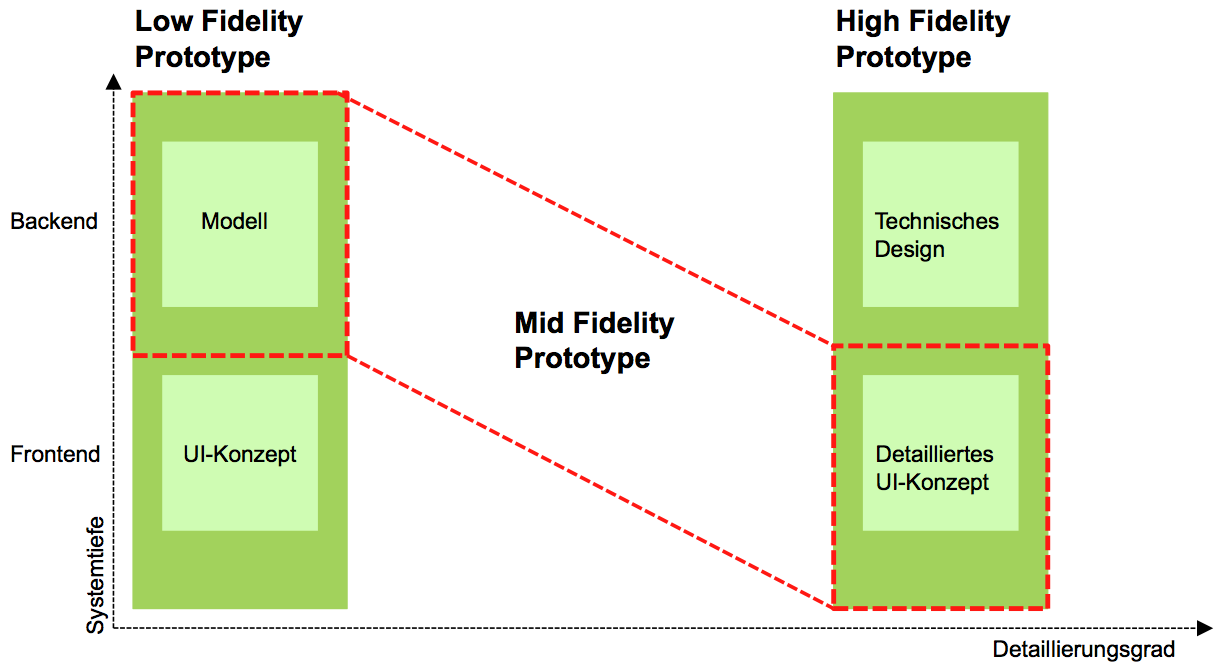
\includegraphics[scale=0.4]{prototyping.png}

\subsection{Low Fidelity Prototype (Low-FI)}
Papier, Storyboards, Skizzen 
\begin{itemize}
	\item[+] Geringe Entwicklungskosten-/zeit
	\item[+] Geeignet für Grobkonzepte
	\item[+] Evaluation von Alternativen
	\item[+] Ideen kommunizieren
	\item[+] Kein technisches Know-How n\"otig
	\item[-]  Kaum Navigation und Interaktion
	\item[-] Eingeschr\"ankte Wiederverwendung
	\item[-] Fehlerbehandlung nicht enthalten
\end{itemize}

\subsubsection{Sketching}
Schnelles Zeichnen mit Papier und Bleistift. \\
Ziel und Zweck:
\begin{itemize}
	\item Ideen für sp\"atere Entwicklung sammeln
	\item Schnelle Visualisierung der Konzepte
	\item Einfaches Kommunikationsmittel
	\item Schnell verbreitet
\end{itemize}

\subsubsection{Balsamiq Mockups}
Tool zum zusammenklicken eines Prototypen. damit kann man schnell und einfach eine Oberfläche skizieren.

\subsubsection{Papier-Prototypen}
Kann verwendet werden, wenn die Funktionalit\"aten bekannt sind. \\
Ziel und Zweck:
\begin{itemize}
	\item Visualisierung der Funktionalit\"at
	\item Aufw\"andiger in der Erstellung als Sketches
	\item Einfach durch Nutzer testbar
	\item Machbarkeits-Test
	\item Unterschiedliches Material (Papier, Post-It
\end{itemize}

\subsection{Mid Fidelity Prototype (Mid-FI)}
HTML, Flash, UI Builders, Wizard of OZ 
\begin{itemize}
	\item[+] Look \& Feel \"ahnlich Endprodukt
	\item[+]  Interaktiv, Navigation
	\item[+] Weiterverwendung m\"oglich
	\item[+] Detaillierte Nutzer-R\"uckmeldung
	\item[-] Mittlere/Hohe Entwicklungskosten/-zeit
	\item[-] Einschr\"ankung der Kreativit\"at
	\item[-] Gefahr der Detailarbeit
\end{itemize}

\subsubsection{Wizard of OZ}
\begin{itemize}
	\item Forschungs-Experiment
	\item Kelley, John F. (1980)
	\item System-Interaktion wird durch einen Menschen simuliert
	\item Beispiel: Sie m\"ochten ein System testen, welches einem Nutzer einen Code per SMS schickt. Dieser Code muss vom Nutzer eingegeben werden, um eine Anmeldung fertig zu stellen. Der Code wird nicht vom System versandt, sondern von einem Menschen.
\end{itemize}

\subsection{High Fidelity Prototype (HI-FI)}
HTML, Flash, UI Builders, Programmierung 
\begin{itemize}
	\item[+] Look \& Feel \"ahnlich Endprodukt
	\item[+] Realistisch, interaktiv, zeitecht
	\item[+] Weiterverwendung m\"oglich
	\item[+] Detaillierte Nutzer-R\"uckmeldung
	\item[-] Hohe Entwicklungskosten/-zeit
	\item[-] Einschr\"ankung der Kreativit\"at
	\item[-] Gefahr der Detailarbeit
\end{itemize}

\section{Horizontale und vertikale Prototypen}

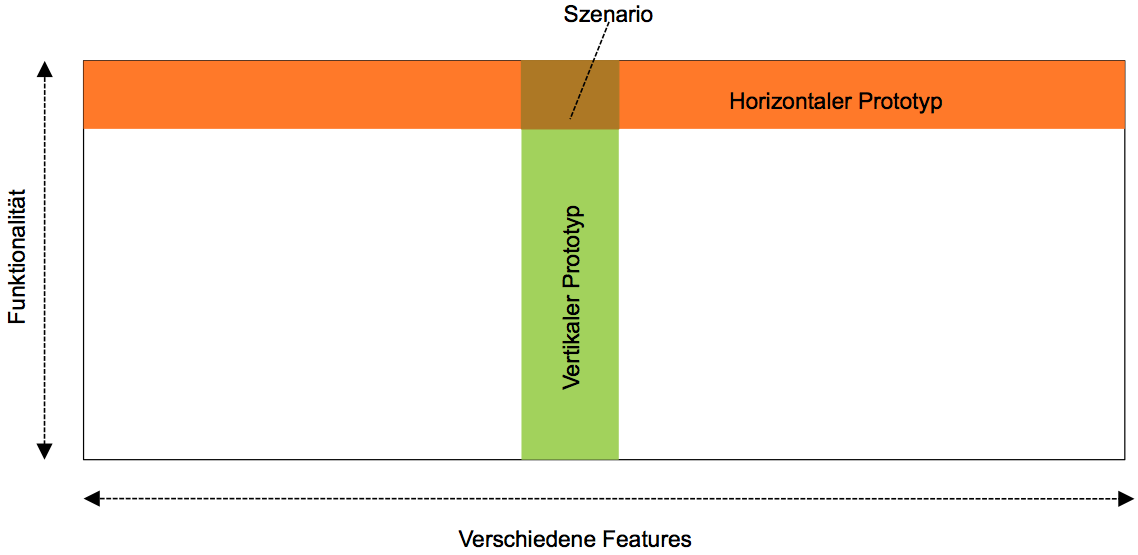
\includegraphics[scale=0.4]{horizontale_vertikale_prototypen.png}

\subsection{Horizontaler Prototyp}
Alle Features, daf\"ur wenig Funktionalit\"at. Beispielsweise das gesamte Interface.

\subsubsection{Evaluation}
\begin{itemize}
	\item der Navigation, des UI-Gesamtkonzeptes
	\item des Zugangs zum System
\end{itemize}
\subsubsection{Verwendung}
\begin{itemize}
	\item In Low-FI und HI-FI
	\item in fr\"uhen Designphasen, um das Feature-Set und das Grobkonzept zu \"uberpr\"ufen
\end{itemize}

\subsection{Vertikaler Prototyp}
Volle Funktionalit\"at für ein paar wenige Features
\subsubsection{Evaluation}
\begin{itemize}
	\item einer einzelnen Funktionalit\"at
	\item des spezifischen Nutzer-Verhaltens
\end{itemize}
\subsubsection{Verwendung}
\begin{itemize}
	\item In HI-FI und (Low-FI)
	\item in fr\"uhen Designphasen um verschiedene Designs einzelner Funktionalit\"aten zu pr\"ufen \"uberpr\"ufen
	\item in sp\"ateren Designphasen, um spezifische Funktionalit\"at zu optimieren
\end{itemize}

\section{UI Builder}
\begin{itemize}
	\item Software, die einem erm\"oglicht, eine grafische Benutzeroberfl\"ache zu entwickeln.
	\item Standardisierte Widgets werden mittels Drag und Drop auf das Interface- Fenster verschoben und dort individuell weiter bearbeitet.
	\item Die Software erzeugt Programmcode.
	\item Eigenst\"andige Applikation oder Teil eines Application Development Systems
	\item GUI-Builder sind ein wesentlicher Bestandteil der modernen Programmierung
\end{itemize}
\subsection{Vorteile}
\begin{itemize}
	\item Wirtschaftlich: Entwicklung, Test und Pflege kann effizienter sein
	\item Qualität des UIs kann profitieren
		\begin{itemize}
			\item Weniger Code schreiben
			\item Verbesserte Modularisierung (Visualisierung von Logik separiert)
			\item Programmier-Expertise im Team darf variieren
			\item Zuverl\"assigkeit des UIs erh\"oht (Code-Generierung)
		\end{itemize}
\end{itemize}
\subsection{Nachteile}
\begin{itemize}
	\item Wirtschaftlich: Entwicklung, Test und Pflege kann erschwert werden
	\item Qualit\"at des UIs kann leiden wenn Builder
		\begin{itemize}
			\item Manuelle Code-\"Anderungen verhindern
			\item Hersteller-spezifische Files verwenden
			\item Die generierte Struktur nicht aufgebrochen werden kann oder nicht zufriedenstellend ist
		\end{itemize}
\end{itemize}

\section{Qualit\"atskriterien}
\begin{description}
	\item[Informationsarchitektur] \hfill \\
		 Info für den User schnell auffindbar? Logisch aufgebaut?
	\item[Navigation] \hfill \\
		 Logische Struktur, Ebenenwechsel, links, oben, klare Titel, Hilfe rechts
	\item[Informationsdarstellung] \hfill \\
		 Klarheit, Konsistenz, Unterscheidbarkeit, Lesbarkeit
	\item[Kompaktheit] \hfill \\
		 Nicht zu kompakt für das Auge, aber dennoch gutes Mass
	\item[Konsistenz] \hfill \\
		 \"Ahnliche Funktionen sich gleich aufrufbar
	\item[Farbgestaltung] \hfill \\
		 Klassifizierung, Auffindbarkeit, Wahrnehmung
	\item[Schriftgestaltung] \hfill \\
		 Zeilenlänge, Zeilenabstand, Buchstabenabstand, Schriftart
	\item[Bildsprache] \hfill \\
		 Blickrichtung, Format, goldene Schnitt, Linien, Kontraste
	\item[Benutzerfu\"uhrung] \hfill \\
		 Aufgabenbez., w\"ahlbar, gut Formuliert, Rückmeldung, Info
\end{description}

\section{Grunds\"atze der Dialoggestaltung}
\begin{description}
	\item[Aufgabenangemessenheit] \hfill \\
		Ein Dialog ist aufgabenangemessen, wenn er den Benutzer unterstützt, seine Arbeitsaufgabe effektiv und effizient zu erledigen.
	\item[Selbstbeschreibungsf\"ahigkeit] \hfill \\
		Ein Dialog ist selbstbeschreibungsf\"ahig, wenn jeder einzelne Dialogschrittdurch R\"uckmeldung des Dialogsystems unmittelbar verst\"andlich ist oder dem Benutzer auf Anfrage erklärt wird.	
	\item[Steuerbarkeit] \hfill \\
		Ein Dialog ist steuerbar, wenn der Benutzer in der Lage ist, den Dialogablauf zu
starten sowie seine Richtung und Geschwindigkeit zu beeinflussen, bis das Ziel erreicht ist.
	\item[Erwartungskonformit\"at:] \hfill \\
		Ein Dialog ist erwartungskonform, wenn er konsistent ist und den Merkmalen des
Benutzers entspricht, z. B. seinen Kenntnissen aus dem Arbeitsgebiet, seiner Ausbildung und seiner Erfahrung sowie den allgemein anerkannten Konventionen.
	\item[Fehlertoleranz] \hfill \\
		Ein Dialog ist fehlertolerant, wenn das beabsichtigte Arbeitsergebnis trotz
erkennbar fehlerhafter Eingaben entweder mit keinem oder mit minimalem Korrekturaufwand seitens des Benutzers erreicht werden kann.
	\item[Individualisierbarkeit] \hfill \\
		Ein Dialog ist individualisierbar, wenn das Dialogsystem Anpassungen an die
Erfordernisse der Arbeitsaufgabe sowie an die individuellen F\"ahigkeiten und Vorlieben des Benutzers zul\"asst.
	\item[Lernf\"orderlichkeit] \hfill \\
		Ein Dialog ist lernf\"orderlich, wenn er den Benutzer beim Erlernen des Dialogsystems unterst\"utzt und anleitet.
\end{description}
\end{document}
